\documentclass[compress]{beamer}
\usetheme{sthlm}

%-=-=-=-=-=-=-=-=-=-=-=-=-=-=-=-=-=-=-=-=-=-=-=-=
%        LOADING BEAMER PACKAGES
%-=-=-=-=-=-=-=-=-=-=-=-=-=-=-=-=-=-=-=-=-=-=-=-=

\usepackage{
booktabs,
datetime,
dtk-logos,
graphicx,
multicol,
pgfplots,
ragged2e,
tabularx,
tikz,
wasysym,
multirow,
float,
caption,
subcaption
}

\pgfplotsset{compat=1.8}

\usepackage[utf8]{inputenc}
\usepackage[portuguese]{babel}
\usepackage[T1]{fontenc}
\usepackage{newpxtext,newpxmath}
\usepackage{listings}

\lstset{ %
language=[LaTeX]TeX,
basicstyle=\normalsize\ttfamily,
keywordstyle=,
numbers=left,
numberstyle=\tiny\ttfamily,
stepnumber=1,
showspaces=false,
showstringspaces=false,
showtabs=false,
breaklines=true,
frame=tb,
framerule=0.5pt,
tabsize=4,
framexleftmargin=0.5em,
framexrightmargin=0.5em,
xleftmargin=0.5em,
xrightmargin=0.5em
}



%-=-=-=-=-=-=-=-=-=-=-=-=-=-=-=-=-=-=-=-=-=-=-=-=
%        LOADING TIKZ LIBRARIES
%-=-=-=-=-=-=-=-=-=-=-=-=-=-=-=-=-=-=-=-=-=-=-=-=

\usetikzlibrary{
backgrounds,
mindmap
}

%-=-=-=-=-=-=-=-=-=-=-=-=-=-=-=-=-=-=-=-=-=-=-=-=
%        BEAMER OPTIONS
%-=-=-=-=-=-=-=-=-=-=-=-=-=-=-=-=-=-=-=-=-=-=-=-=

\setbeameroption{show notes}

%-=-=-=-=-=-=-=-=-=-=-=-=-=-=-=-=-=-=-=-=-=-=-=-=
%        BEAMER COMMANDS
%-=-=-=-=-=-=-=-=-=-=-=-=-=-=-=-=-=-=-=-=-=-=-=-=


%-=-=-=-=-=-=-=-=-=-=-=-=-=-=-=-=-=-=-=-=-=-=-=-=
%
%	PRESENTATION INFORMATION
%
%-=-=-=-=-=-=-=-=-=-=-=-=-=-=-=-=-=-=-=-=-=-=-=-=

\title{Algoritmos de eleições}
\subtitle{DCE540 - Computação Paralela e Distribuída}
%\date{\small{\jobname}}
\author{\texttt{Iago Carvalho}}
\institute{\texttt{Departamento de Ciência da Computação}}

\hypersetup{
pdfauthor = {Iago A. Carvalho},      
pdfsubject = {Computação Paralela e Distribuída},
pdfkeywords = {},  
pdfmoddate= {D:\pdfdate},          
pdfcreator = {WriteLaTeX}
}

\begin{document}

\begin{frame}
\titlepage

\end{frame}

%% --------------------------------------------------------

\begin{frame}{Eleições}

Alguns algoritmos de sincronização e coordenação precisam definir um processo que atue como coordenador
\begin{itemize}
    \item É possível ter um processo especial com esta tarefa
    \item Também é possível escolher um processo, dentre os existentes, para atuar como coordenador
\end{itemize}

\vspace{0.5cm}

A forma mais simples de escolher um processo como coordenador é com a utilização de um algoritmo de eleições!
\begin{itemize}
    \item Algoritmo de \textit{bully}
    \item Algoritmo de anel
\end{itemize}
\end{frame}

%% --------------------------------------------------------

\begin{frame}{Algoritmo de bully}

\centering 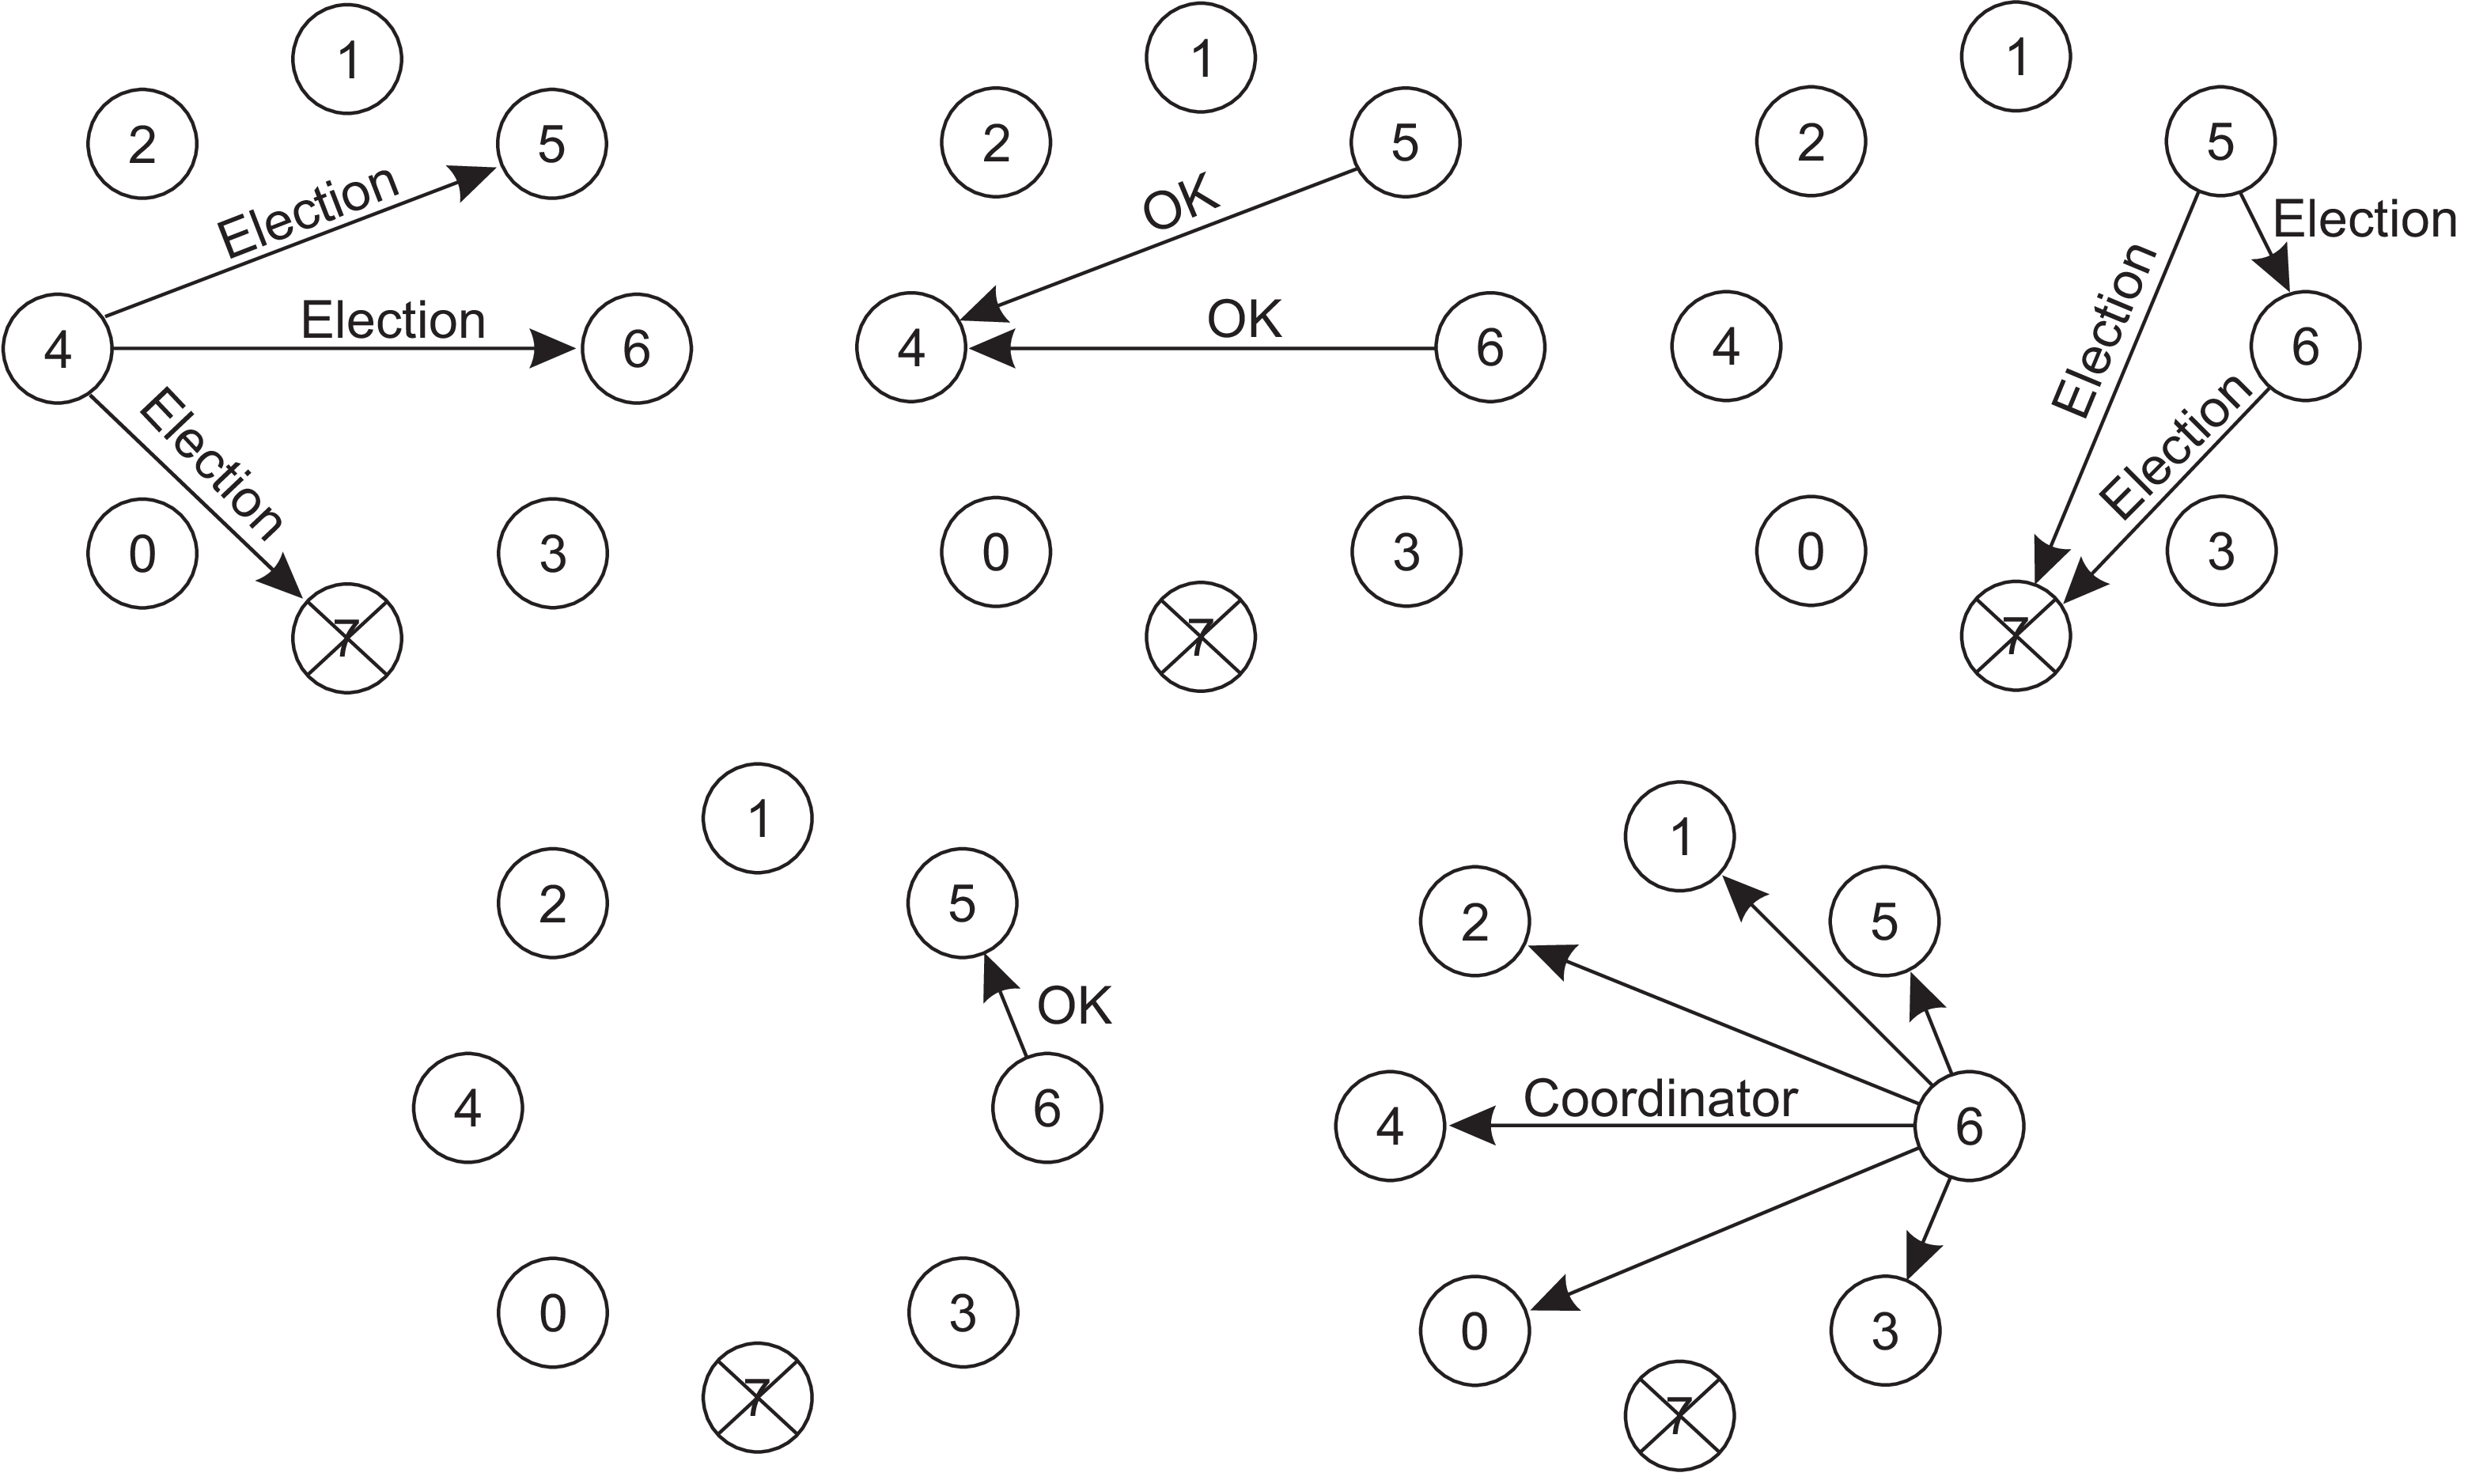
\includegraphics[width=\textwidth]{images/bully.png}
\end{frame}

%% --------------------------------------------------------

\begin{frame}{Algoritmo do anel}

\centering 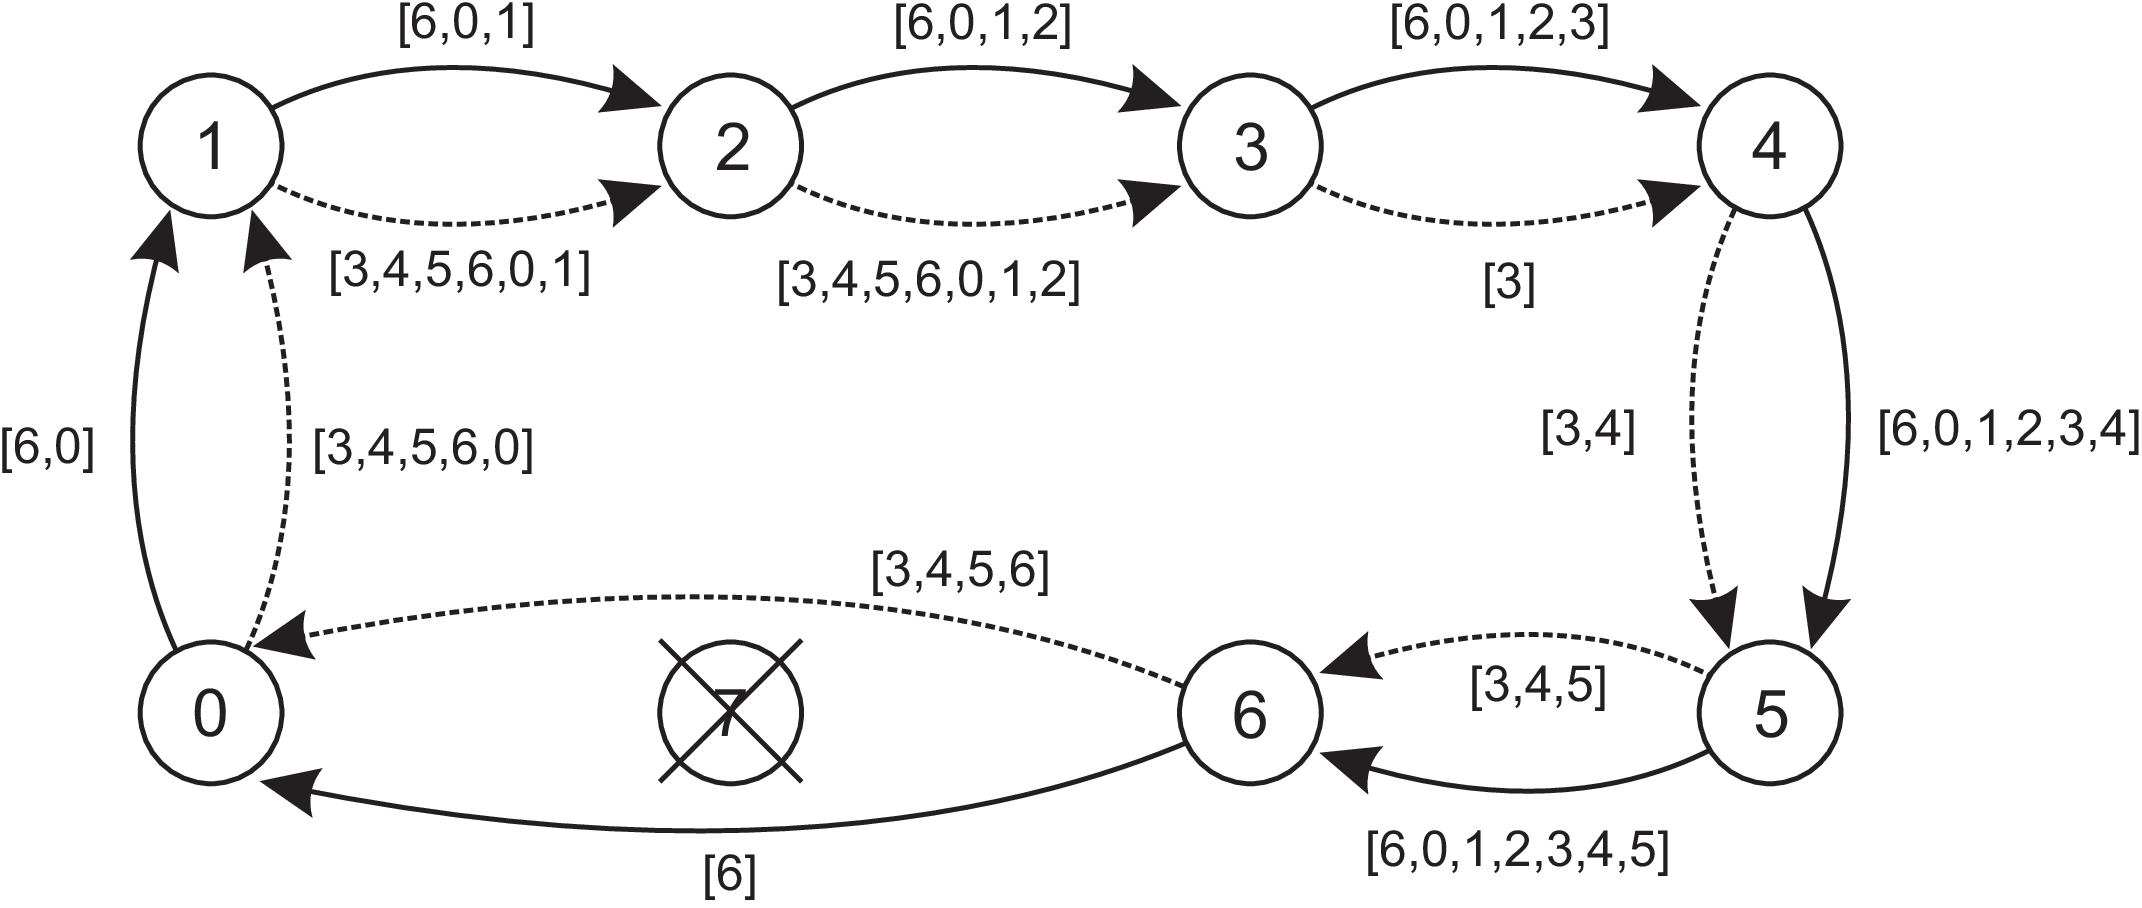
\includegraphics[width=\textwidth]{images/ring.png}

\end{frame}

%% --------------------------------------------------------

\begin{frame}{Eleições em redes P2P de larga escala}

O algoritmo de bully e o algoritmo do anel não funcionam muito bem para sistemas muito grandes
\begin{itemize}
    \item Muitos nós para coordenar
    \item Muitas mensagens são necessárias
\end{itemize}

\vspace{0.5cm}

Assim, em sistemas de larga escala, é comum termos diversos processos coordenadores

\vspace{0.5cm}

Em redes P2P, processos coordenadores são chamados de super usuários

\end{frame}

%% --------------------------------------------------------

\begin{frame}{Eleições em redes P2P de larga escala}

A escolha de super usuários deve levar em consideração 4 requisitos:
\begin{enumerate}
    \item Usuários normais devem ser capazes de se comunicar com super-usuários de forma rápida (baixa latência)
    \item Super usuários devem estar distribuidos uniformemente pela rede
    \item Deve existir um número mínimo de super usuários
    \begin{itemize}
        \item Número é proporcional a quantidade total de usuários
    \end{itemize}
    \item Cada super usuário tem um limite superior de quantos usuários ele consegue atender
\end{enumerate}

\end{frame}

%% --------------------------------------------------------

\begin{frame}{Eleições em redes P2P de larga escala}

Estes 4 requisitos podem ser atingidos de maneira relativamente fácil
\begin{itemize}
    \item Redes estruturadas
    \item Redes não estruturadas aleatórias
\end{itemize}

\end{frame}

%% --------------------------------------------------------

\begin{frame}{Eleições em redes P2P não estruturadas}

\vspace{1cm}

\centering 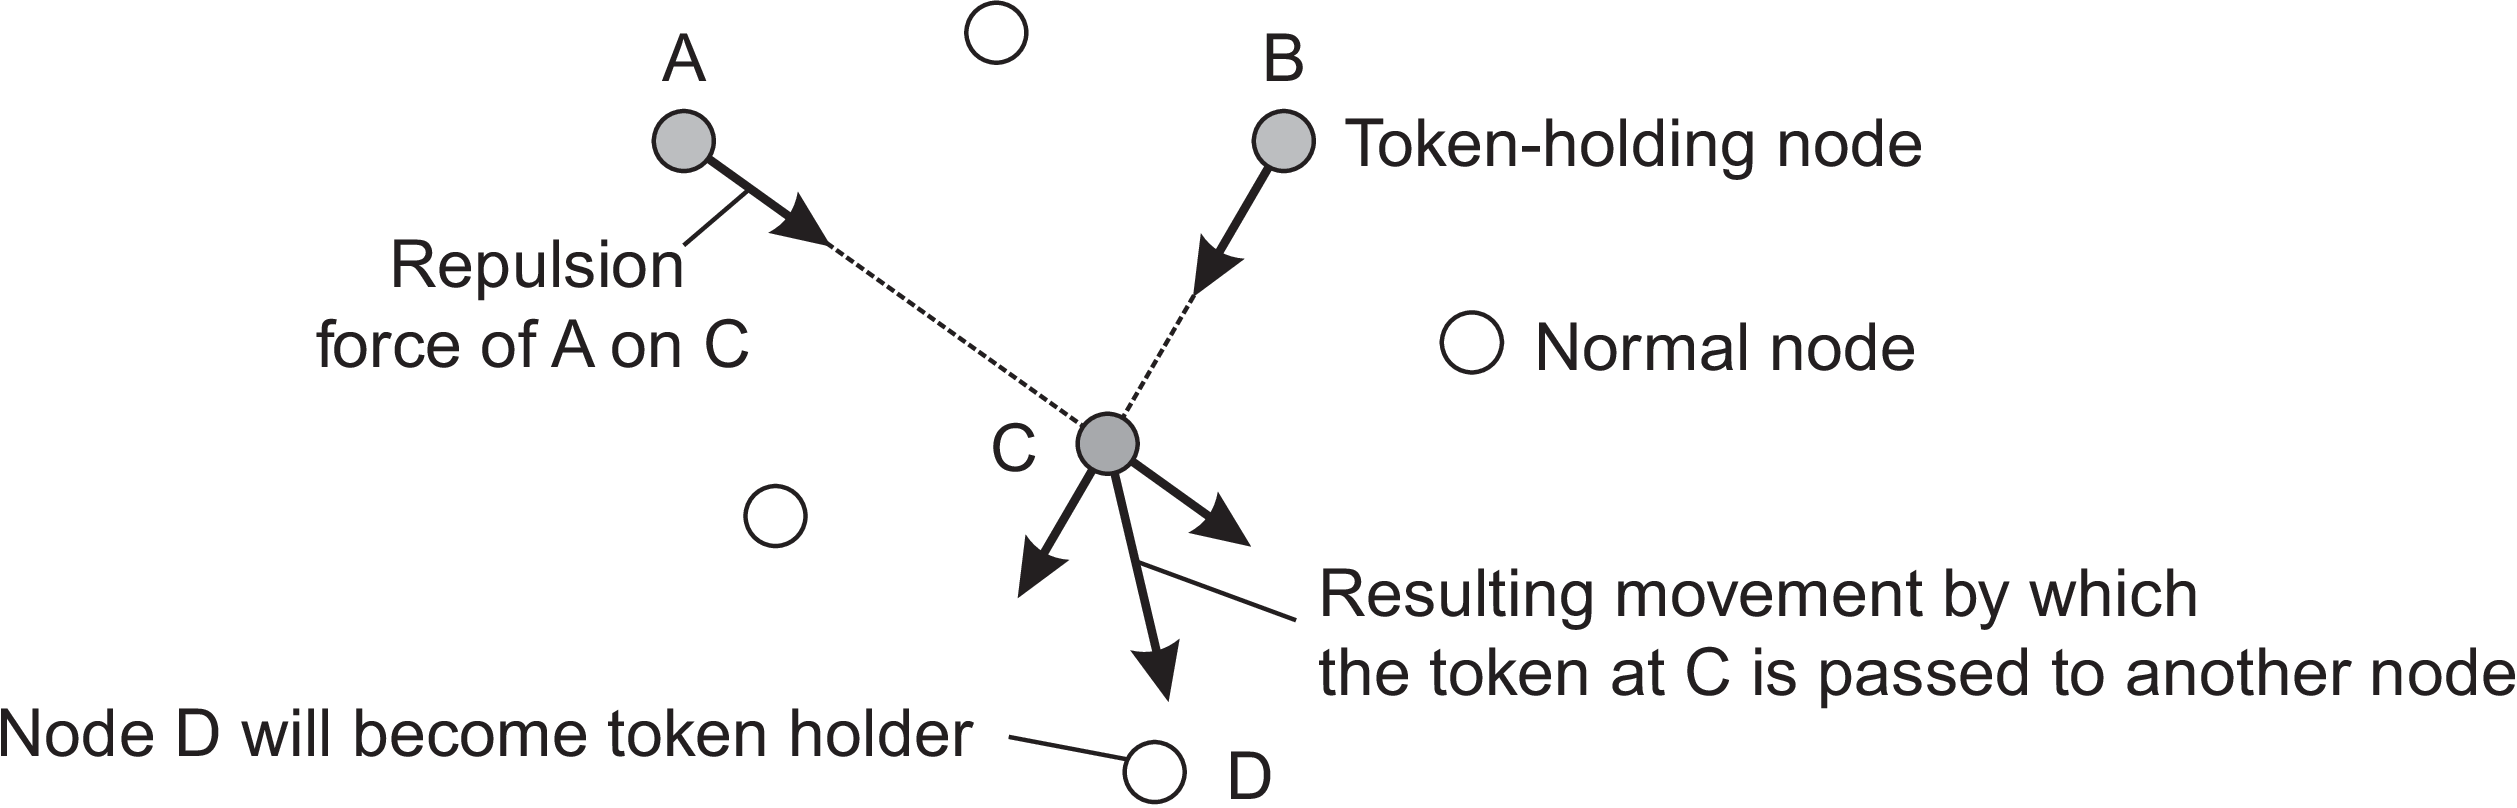
\includegraphics[width=\textwidth]{images/nao-estruturadas.png} 
\end{frame}

\end{document}
